\documentclass[12pt,a4paper]{article}
\usepackage[utf8]{inputenc}
\usepackage[spanish]{babel}
\usepackage{amsmath}
\usepackage{amsfonts}
\usepackage{amssymb}
\usepackage{graphicx}
\usepackage{array,tabularx}
\usepackage[left=2cm,right=2cm,top=2cm,bottom=2cm]{geometry}
\begin{document}
	\begin{titlepage}
	\begin{center}
		{\huge \textbf{Universidad Veracruzana}}\\
		\vspace{2cm}  
		{\Large {Documento de descripcion}}\\
		\vspace{5mm}	
		{\Large {Instagram}}\\
		\begin{figure}[h]
			\centering
			
\includegraphics[scale=0.10]{uvlogo}
		\end{figure}
		{\Large {Ingeniería de software}}\\
		\vspace{2cm}
		{\Large {Gerardo Iván Martínez Espinosa}}\\
		\vspace{25mm}	
		\rule{8cm}{0.5mm} \\ \Large Vo.bo\\ 
	\end{center}
\end{titlepage}
	\vspace{1 cm}
	\section{Introduccion}
	
	La pagina instagram fue creada con react y firebase como medio de almacenamiento, te permite subir fotos e interactuar con ellos. Instagram se basa en una red social del mismo nombre que permite subir fotos e interactuar con otros usuarios y sus fotos.\\
	
	\section{Login}
	Te permite .ingresar con tu cuenta de facebook, al hacerlo se crea tu perfil automaticamente\\
	
	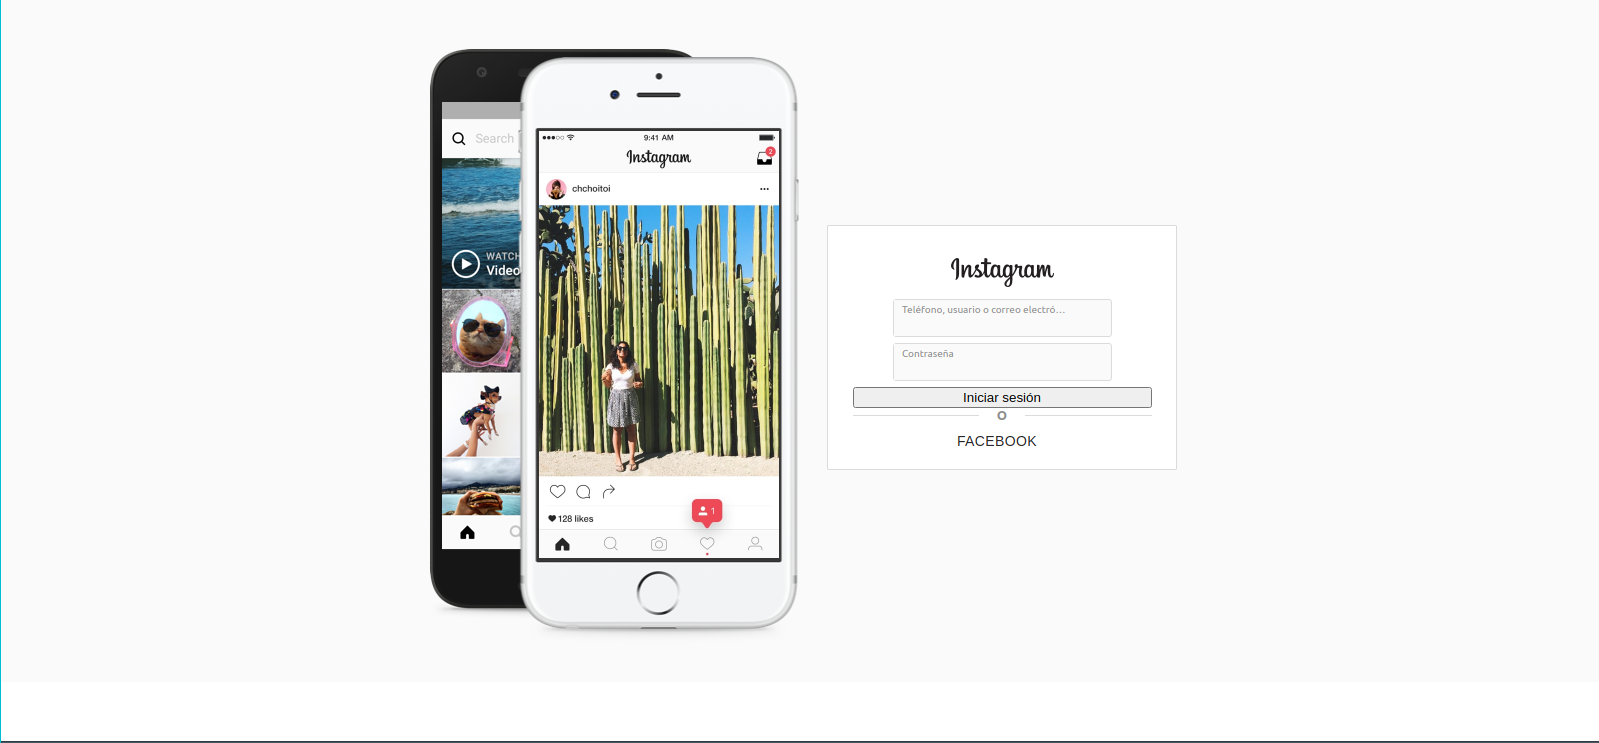
\includegraphics[scale=0.20]{Login}
	
	\section{Inicio}
	Al acceder con una cuenta de facebook, en el inicio de la pagina se puede ver un header que contiene las opciones de ver perfil, subir una nueva foto, ir a la pagina principal. En la parte de perfil se encontraran todos los posts creados por el usuario. Finalmente en la parte de posterior derecha contaremos con la opción de poder crear un nuevo post.\\
	
	\includegraphics[scale=0.20]{Inicio1}	
	
	
	\section{Perfil}
	Una vez creado el nuevo post se puede ver  en la sección de perfil donde se le puede dar like o agregar un comentario.
	
	\includegraphics[scale=0.20]{Perfil}
	
\end{document}